\documentclass[acmtog]{acmart}
\usepackage{graphicx}
\usepackage{subfigure}
\usepackage{natbib}
\usepackage{listings}
\usepackage{bm}
\usepackage{soul}
\usepackage{algorithm}
\usepackage{algorithmic}

\definecolor{blve}{rgb}{0.3372549 , 0.61176471, 0.83921569}
\definecolor{gr33n}{rgb}{0.29019608, 0.7372549, 0.64705882}
\makeatletter
\lst@InstallKeywords k{class}{classstyle}\slshape{classstyle}{}ld
\makeatother
\lstset{language=C++,
	basicstyle=\ttfamily,
	keywordstyle=\color{blve}\ttfamily,
	stringstyle=\color{red}\ttfamily,
	commentstyle=\color{magenta}\ttfamily,
	morecomment=[l][\color{magenta}]{\#},
	classstyle = \bfseries\color{gr33n}, 
	tabsize=2
}
\lstset{basicstyle=\ttfamily}

% Title portion
\title{Assignment 1 Part 1:\\ {Traditional Light Field Rendering}}

\author{Name:\quad Chenqihe  \\ student number:\ 2020533088
\\email:\quad chenqh@shanghaitech.edu.cn}

% Document starts
\begin{document}
\maketitle

\vspace*{2 ex}

\section{Introduction}
	\quad In this assignment, we implement novel-view synthesis results based on traditional light field rendering. 
	
	\quad There are more concrete problems that have been solved. 
	
	\begin{itemize}
		\item Implement both bilinear and quadra-linear interpolation schemes to interpolate views along $x$ and $y$ directions.
		
		\item Implement focussing and defocussing by variable focal planeand variable aperture size.
		
		\item Implement the z-directional motion of the camera by expanding field of view.
		
	\end{itemize}
	
\section{Related work}
\quad In this section, we review related work to provide context for our own work.

\textbf{Plen-optic Function} Traditional plen-optic functionis defined by 7D that $(x, y, z, \theta, \phi, \lambda, t)$. In this assignment, we assume that camera receives the light rays. $(x, y, z)$ is where light hits, i.e.3D coordinates of pixels on the camera's focal plane. $(\theta, \phi)$ is the direction of light ray, i.e. how light rays hit the focal plane. $(\lambda)$ is the wavelength of light ray, i.e. the information of illumination. $(t)$ is the time spot, i.e. describes how the radiance changes during the timespan.

\textbf{Light field} It describes a simple and robust method for generating new views from abitrary(but actually limited) camera positions without depth information or feature matching, simply by combing and resampling the available images.

\quad The key to this technique lies in interpreting the input images as 2D slices of a 4D function. The solution it proposes is to parameterize lines by their intersections with two planes in arbitrary position. In other words, it simplifies the plen-optic function from 7D into 4D.

\section{Methods}

\subsection{Representation of rays: light slab}
	\quad In traditional light field, we use a light slab to parameterize rays by $(s, t, u, v)$, where $(s, t)$ is the index of camera, $(u, v)$ is the index of pixel aof $(s,t)$ camera. Thus, we store all the images information or color of rays into a 4D matrix.

\begin{figure}[h]
	\centering
	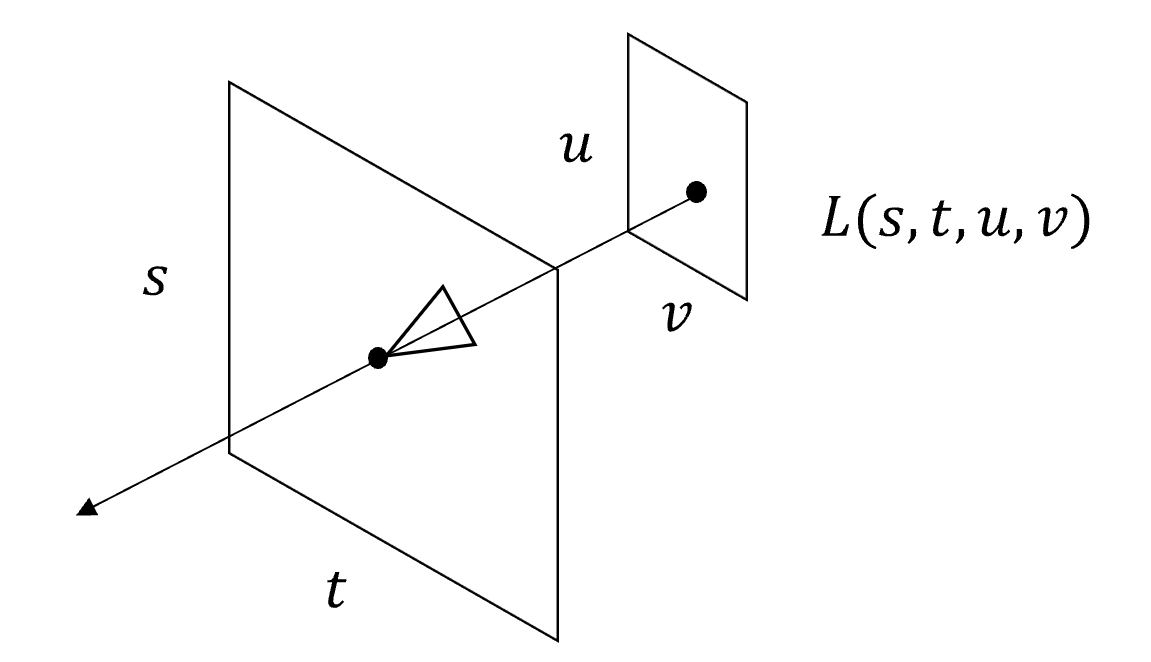
\includegraphics[scale=0.14]{light slab.png}
	\caption{light slab}
	\label{fig:Fig1}
\end{figure}

 \quad In light slab, an oriented line is defined by a directional line from a point on $uv$ plane to a point on $st$, where $st$ plane is camera plane, $uv$ plane is focal plane.
 
 \quad In this way, we compress all the input images into a 4D expression $(s, t, u, v)$.
 
 \subsection{Rendering}
 \subsubsection{Disparity}
 	\quad A point $(u,v)$ on focal plane can be exactly mapped back to a 3D point in world space. To render an image at the view of a virtual camera, any points on focal plane should be consistent in the existing cameras. Please notice that the locations should be consistent on 3D world space, but may not be on the 2D focal plane. The reason why 2D focal plane may not be consistent can be explained by below:
 	
 	\quad Consider a light slab $(s, t, u, v)$ and a 3D point $P$ $(x,y,z)$ lies inside the light slab. A problem is how to get all the light rays in light slab that pass throught $P(x,y,z)$.
 	
 	\quad Know conditions: 3D point P$(x,y,z)$,  $st$ plane $\{(s, t, 0) | (s,t)\in[0, 1]^2\}$, $uv$ plane $\{(u, v, 1)| (u,v)\in[0, 1]^2\}$
 	
 	\quad Assume the target light ray intersects $st$ plane at point $(s, t, 0)$ and $uv$ plane at point $(u, v, 1)$, then the origin of light ray $\dot{o}=(u,v,1)$, the direction of light ray (not normalized) $\vec{d}=(s-u, t-v ,-1)$, i.e. $r(\lambda)=\dot o+ \lambda \vec{d}$
 	
 	\[
 	r(\lambda)=(u, v, 1) + \lambda(s-u, t-v, -1)
 	\]
 	
 	 \quad since $P(x,y,z)$ is on the light ray, we have
 	 
 	 \[
		\begin{cases}
			x &= (1-\lambda)u+\lambda s\\
			y &= (1-\lambda)v+\lambda t\\
			z &= 1-\lambda
		\end{cases}
 	 \]
 	 
	\quad Using $\lambda=1-z$, we have
	
	\[
		\begin{cases}
			zu - (1-z)s &= x \\
			zv - (1-z)t &= y
		\end{cases}
	\]
	\quad Thus, we construct equations w.r.t $u\sim s$ and $v\sim t$, then assume we have a camera array $st$ plane, and each integer point corresponds to a single camera. If each cameras have the same interval distance along $s,t$ directions respectively, the transform of $st$ focal plane is contant. And we define the constant by $\delta$, and we regard $\delta$ as disparity, which reflects how $uv$ changes w.r.t $st$.
	
	\begin{figure}[h]
		\centering
		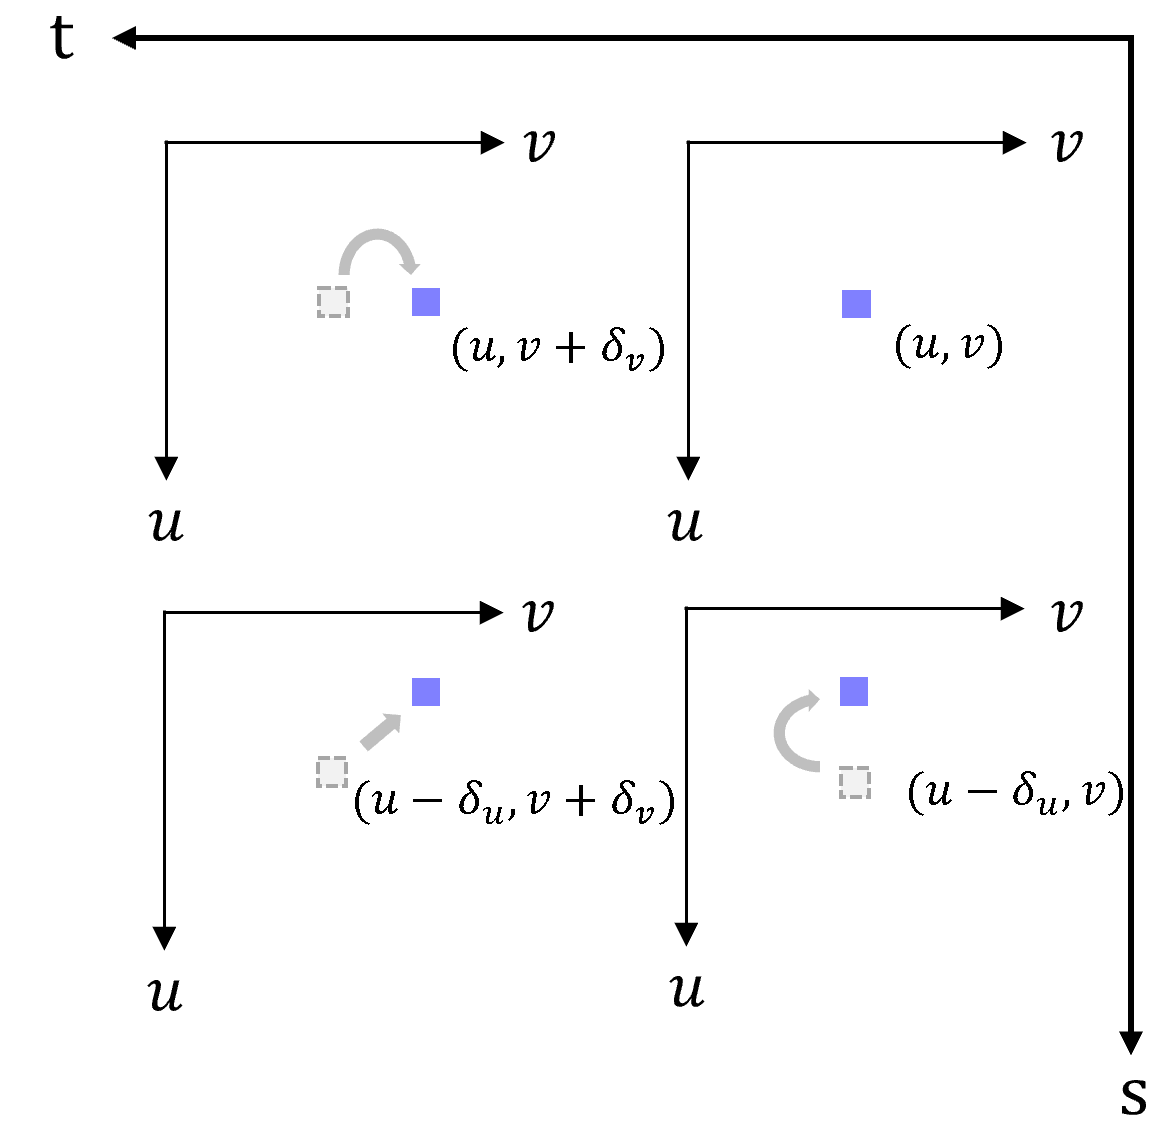
\includegraphics[scale=0.14]{disparity.png}
		\caption{disparity}
		\label{fig:Fig2}
	\end{figure}

	\quad In Fig.\ref{fig:Fig2}, we show four neighbor cameras and describe how to align pixel w.r.t disparity. Generally, for a camera array, the disparities along $s$ and $t$ direction are the same. However, we'd better check it manually. And we check that it is exactly true for dataset in this assignment.
	
	\subsection{Interpolation}
	\quad In general, there are two steps to complete interpolation. First, we interpolate the images of neighbor cameras w.r.t. disparity. Second, we interpolate pixel value for each image, respectively. 
		 
	\quad We implement two ways for interpolation, i.e. bilinear and quadra-linear. Bilinear interpolation only interpolates on $st$ plane i.e. multi-camera interpolation. Quadra-linear interpolation interpolates both $st$ plane and $uv$ plane, that is two bilinear interpolation actually.
	
	\quad To implement bilinear interpolation, we display a virtual camera at $(s,t)$ and $s,t$ can be floating number, which implies that we can not directly get the results from existing $(s,t,u,v)$. Because all cameras in $(s,t,u,v)$ light field are all at integer points.Thus, we apply bilinear interpolation w.r.t $(s,t)$'s neighbor cameras. 
	
	\begin{figure}[h]
		\centering
		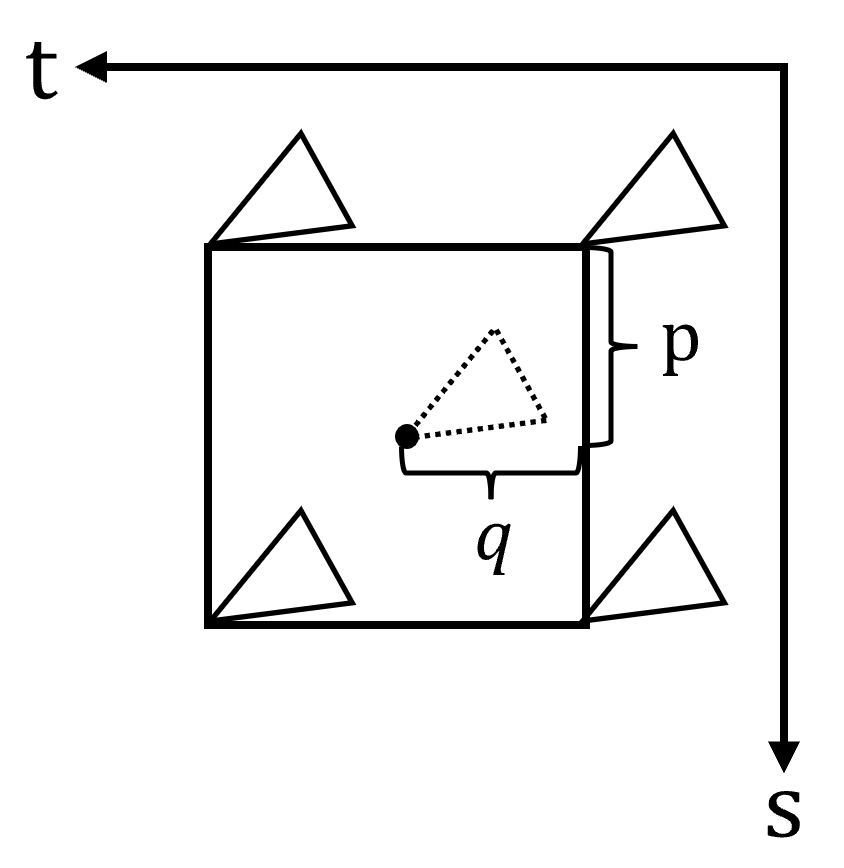
\includegraphics[scale=0.16]{bilinear interpolation.png}
		\caption{bilinear interpolation}
		\label{fig:Fig3}
	\end{figure}
	
	\quad In fact, bilinear interpolation calculates the weights to sum up the images of neighbor camera. For a virtual camera, we get four neighbor cameras' views that are shifted by disparity. And we first interpolates along $s$ axis and second interpolates along $t$ axis.
	
	\quad Assume virtural camera is at $(s^\prime, t^\prime)$, then the righttop camera is at $(s,t)$, where $s=floor(s^\prime), t=floor(t^\prime)$. For simplifity, we denote righttop camera by $C(0,0)$. The other three cameras are $C(0, 1)$, $C(1, 1)$, $C(1, 0)$ in anticlockwise order.
	
	\quad First, interpolate along $s$ axis, we have 
	\[
	\begin{aligned}
		C_0 &= pC(1, 0) + (1-p)C(0, 0) \\
		C_1 &= pC(1, 1) + (1-p)C(0, 1)
	\end{aligned}
	\]
	
	\quad Second, interpolate along $t$ axis, we gave
	
	\[
	\begin{aligned}
		C(s^\prime, t^\prime) &= qC_1 + (1-q)C_0 \\
		&= (1-p)(1-q)C(0,0) + (1-p)qC(0,1)   \\
		&+ p(1-q)C(1,0) + pqC(1,1)
	\end{aligned}
	\]
	
	\quad Therefore, we complete the bilinear interpolation w.r.t neighbor cameras. Generally, we can also adapt it to calculating the interpolation of pixels on $uv$ plane, which is needed in quadra-linear interpolation method.

	\begin{figure}[htbp]
		\centering
		
\includegraphics[scale=0.5]{bilinear.png}
		\caption{bilinear result}
		\label{fig:Fig4}
	\end{figure}

	\begin{figure}[htbp]
		\centering
		
\includegraphics[scale=0.5]{quadra-linear.png}
		\caption{quadra-linear result}
		\label{fig:Fig5}
	\end{figure}

	\subsection*{What do you observe if you use biliner interpolation on undersampled light field?}
	\quad Aliasing artefacts. 
	
	\begin{figure}[htbp]
		\centering
		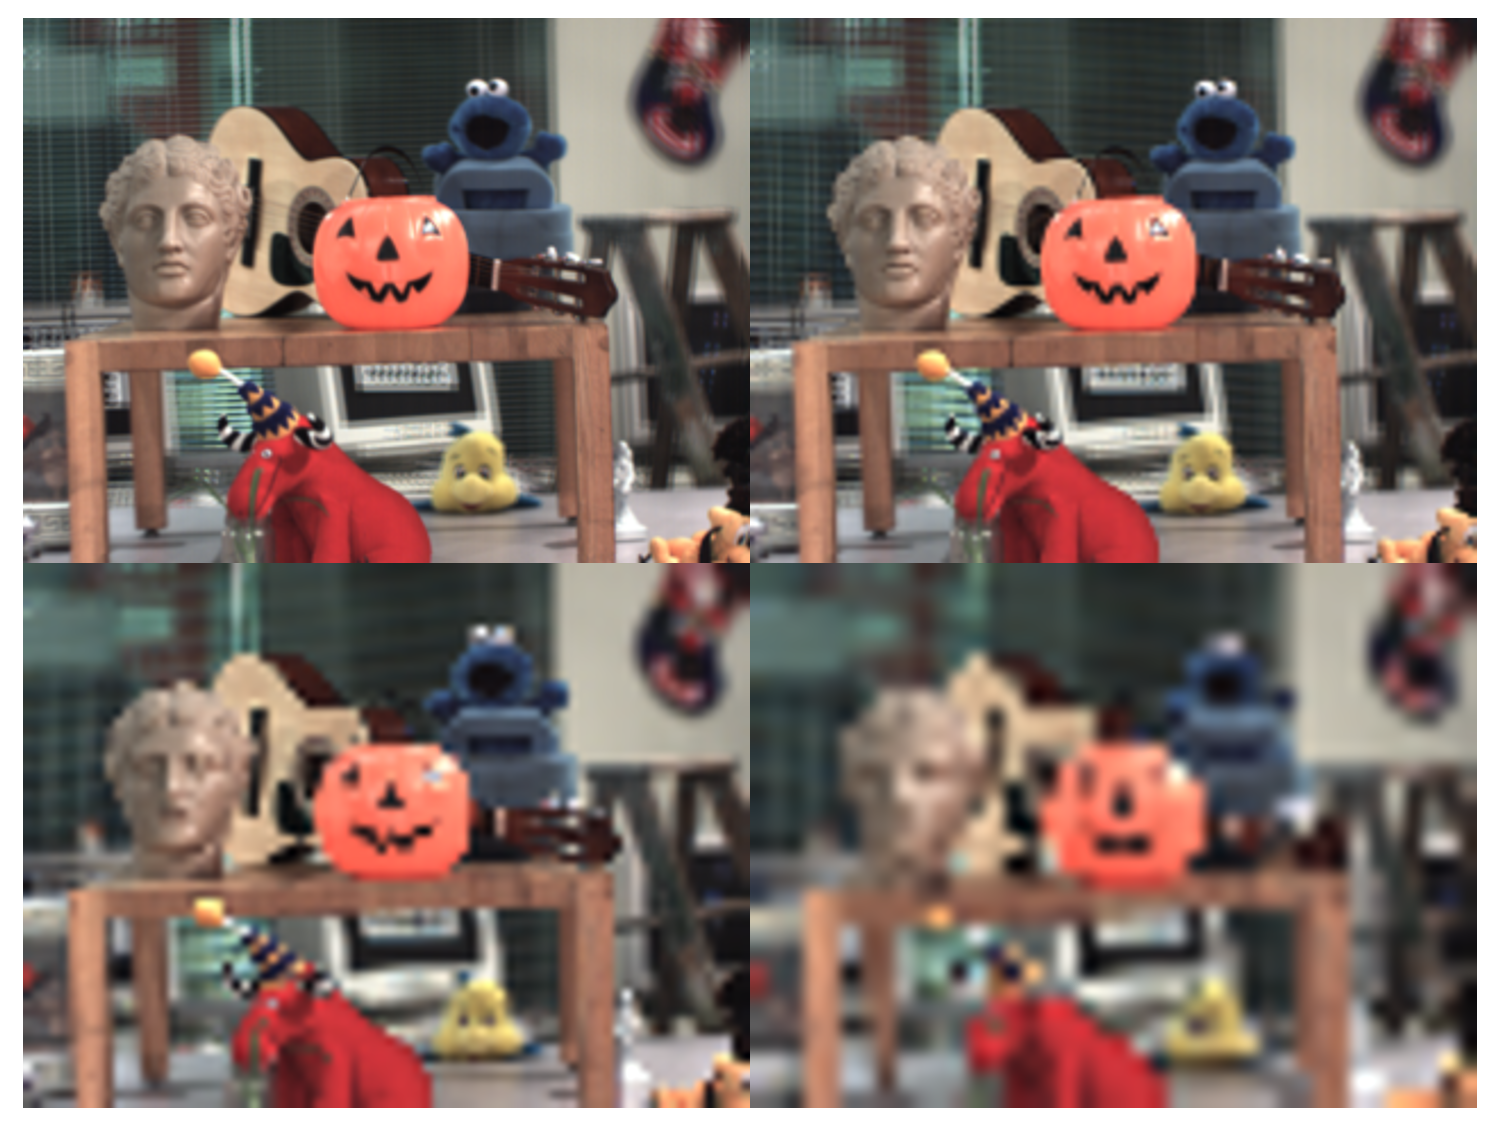
\includegraphics[scale=0.15]{undersampled.png}
		\caption{undersampled result by bilinear}
		\label{fig:Fig6}
	\end{figure}

	\subsection{Variable focal plane}
	\quad We achieve the effect of variable focal plane by mapping the depth $z$ of the focal plane to the disparity. Just like what we show in the disparity part, we conclude the equation w.r.t disparity and depth by $\delta=\frac{1-z}{z}$.
	
	\subsection*{What happens when you move your focal plane from far to near?}
		\quad When the focal plane is far, the scene becomes very blurry. As focal plane gets closer and closer, we can see the background of scene clearly and the objects clearly soon. However, when focal plane gets too close, the scene becomes blurry and has some invisible black areas. 
		
		\quad The reason behind this phenomenon is that the area that we can see clearly in the scene depends on disparity. One value of $z$ corresponds to one value of disparity and one focal plane. The closer the focal plane is, the bigger the disparity is. Thus, we can see part of the scene clearly only at an appropriate range of disparity or depth of focal plane.
		
	
		\begin{figure}[htbp]
			\centering
			\subfigure[focal plane at $z=0.500$]{
\includegraphics[scale=0.3]{focal_plane_0.5000.png}
				\label{fig:Fig7}}
			\quad
			\subfigure[focal plane at $z=0.400$]{
\includegraphics[scale=0.3]{focal_plane_0.4000.png}
				\label{fig:Fig8}}
			\quad
			\subfigure[focal plane at $z=0.300$]{
\includegraphics[scale=0.3]{focal_plane_0.3000.png}
				\label{fig:Fig9}}
			\quad
			\subfigure[Stockings at $z=0.200$]{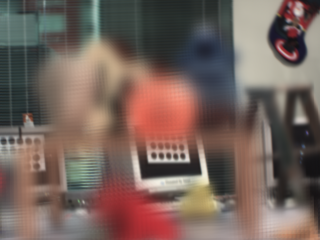
\includegraphics[scale=0.3]{stocking 0.200.png}
				\label{fig:Fig10}}
			\quad
			\subfigure[Computerat $z=0.190$]{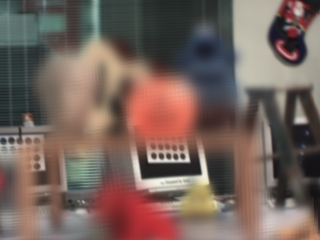
\includegraphics[scale=0.3]{computer 0.190.png}
				\label{fig:Fig11}}
			\quad
			\subfigure[Blue frog at $z=0.118$]{
\includegraphics[scale=0.3]{blue frog 0.118.png}
				\label{fig:Fig12}}
			\quad
			\subfigure[Pumpkin at $z=0.111$]{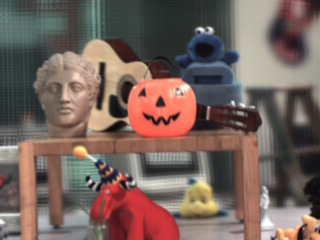
\includegraphics[scale=0.3]{pumpkin 0.111.png}
				\label{fig:Fig13}}
			\quad
			\subfigure[Red bull at $z=0.105$]{\includegraphics[scale=0.3]{Red bull 0.105.png}
				\label{fig:Fig14}}
			\quad
			\subfigure[focal plane at $z=0.090$]{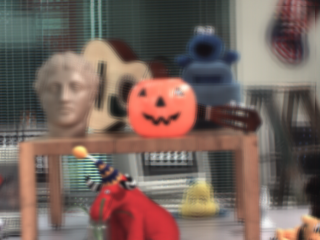
\includegraphics[scale=0.3]{focal_plane_0.0900.png}
				\label{fig:Fig15}}
			\quad
			\subfigure[focal plane at $z=0.050$]{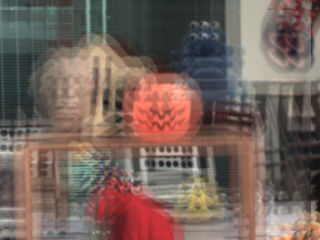
\includegraphics[scale=0.3]{focal_plane_0.0500.png}
			\label{fig:Fig16}}
			\caption{Variable focal plane from far to near}
		\end{figure}

	
	\subsection*{Which focal plane gives yo the optimal results(least aliased reconstruction)?}
	\quad $z=\frac{1}{9}$

	\subsection{Variable aperture size}
		\quad We implement a wide aperture filter to show the effect of changing aperture size. In fact, when aperture size $=1$, it corresponds to bilinear or quadra-linear interpolation. However, when aperture size $>1$, we have to deal with with Gaussian weigh. Let aperture size be $a$ and the weight for a neighbor camera is that 
		
		\[
		w(s, t) = \exp(-\Vert\delta(s, t)\Vert_2^2 / (2a^2))
		\]
		
		\quad After calculating all weights of neighbor camera, we need to normalize the sum to $1$.
		
		\[
		w^\prime(s,t) = \frac{w(s, t)}{\sum w(s,t)}
		\]
		
		\quad We show the results of stockings at $z=0.200$ by variable aperture size. And we find that we can see  the stockings clearly while seeing other things unclearly with a big aperture.
		
		\begin{figure}[htbp]
			\centering
			\subfigure[aperture size $=1$]{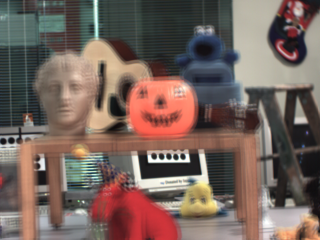
\includegraphics[scale=0.3]{aperture_size_1_2.png}
				\label{fig:Fig17}}
			\quad
			\subfigure[aperture size $=2$]{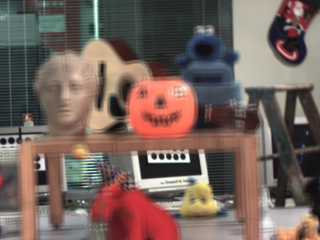
\includegraphics[scale=0.3]{aperture_size_2_2.png}
				\label{fig:Fig18}}
			\quad
			\subfigure[aperture size $=3$]{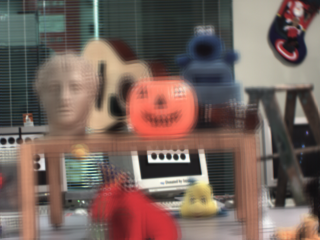
\includegraphics[scale=0.3]{aperture_size_3_2.png}
				\label{fig:Fig19}}
			\quad
			\subfigure[aperture size $=4$]{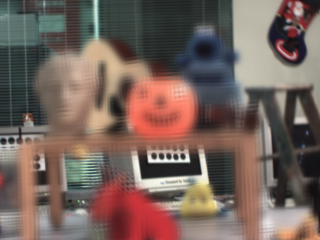
\includegraphics[scale=0.3]{aperture_size_4_2.png}
				\label{fig:Fig20}}
			\quad
			\subfigure[aperture size $=5$]{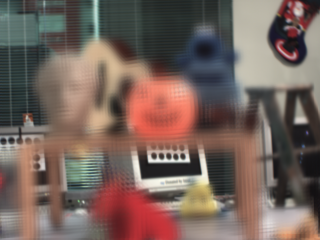
\includegraphics[scale=0.3]{aperture_size_5_2.png}
				\label{fig:Fig21}}
			\quad
			\subfigure[aperture size $=6$]{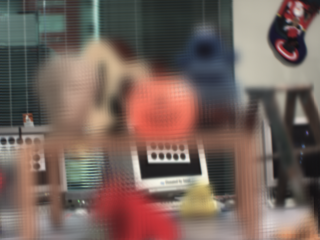
\includegraphics[scale=0.3]{aperture_size_6_2.png}
				\label{fig:Fig22}}
			\quad
			\subfigure[aperture size $=7$]{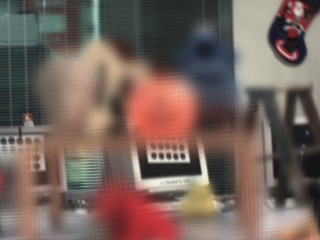
\includegraphics[scale=0.3]{aperture_size_7_2.png}
				\label{fig:Fig23}}
			\quad
			\subfigure[aperture size $=8$]{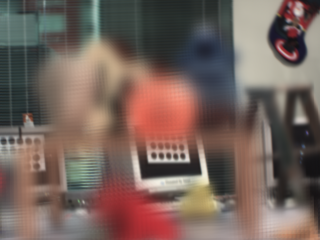
\includegraphics[scale=0.3]{aperture_size_8_2.png}
				\label{fig:Fig24}}
			\caption{Variable aperture size with focal plane $z=0.200$ }
		\end{figure}
	
		\subsection*{What happens when you increase the size of the aperture?}
			\quad With the size of aperture increasing, we implement the focussing effect and we can only see the objects at the specific depth clearly.
			
		\subsection{Expand field of view}
			\quad We implement the z-directional motion of the camera w.r.t the depth of virtual camera. When the virtual camera is on the camera array plane, the depth is $0$. However, the depth of the virtual camera increases when it goes towards the focal plane or the scene.
			
			Assume that $z>=0$ when the virtual camera gets closer to the scene. Then we can calculate the projection region onto the image captured by the virtual camera on the camera array plane. Denote the focal plane by $f$.
			
			\[
			\begin{aligned}
				U^\prime &= U * (f-z)/z \\
				V^\prime &= V * (f-z)/z
			\end{aligned}
			\]
			
			Then, we can get the new image by upsampling the original image in the projection region.
			\begin{figure}[htbp]
				\centering
				\subfigure[depth $=0.00$]{
\includegraphics[scale=0.3]{depth_0.000.png}
					\label{fig:Fig25}}
				\quad
				\subfigure[depth $=0.02$]{
\includegraphics[scale=0.3]{depth_0.020.png}
					\label{fig:Fig26}}
				\quad
				\subfigure[depth $=0.03$]{
\includegraphics[scale=0.3]{depth_0.030.png}
					\label{fig:Fig27}}
				\quad
				\subfigure[depth $=0.04$]{
\includegraphics[scale=0.3]{depth_0.040.png}
					\label{fig:Fig28}}
				\quad
				\subfigure[depth $=0.05$]{
\includegraphics[scale=0.3]{depth_0.050.png}
					\label{fig:Fig29}}
				\quad
				\subfigure[depth $=0.07$]{
\includegraphics[scale=0.3]{depth_0.070.png}
					\label{fig:Fig30}}
				\quad
				\caption{Expand field of view with focal plane $z=0.111$ }
			\end{figure}
\end{document}
